\subsection{Parallel computing experiments}

Because one of the most crucial points of SMODERP2D computations is
the speed, an experimental branch allowing (both CPU and GPU-based)
parallelized computations has been developed.

The main step was to rewrite all loop-based computations into
matrix-based mathematical operations. To keep matrices as so-called
tensors and to perform all the operations, an open source  TensorFlow Python
library \cite{tensorflow2015-whitepaper} developed by Google Brain
Team\footnote{https://ai.google/research/teams/brain/} was used. Even though
TensorFlow is most widely used for machine learning
and its performance on basic mathematical operations is not always better
than the one of NumPy (a quick comparison with NumPy and Numba can be
seen in \cite{tf-np}), it had been preferred for its easy switch
between CPU and GPU-based core (it depends only on the version of
TensorFlow the user has installed, no needs for changes in the code) and
therefore support also for users without an access to machines with
GPU. Another advantage of TensorFlow is its usage of so-called
graphs. A graph is a representation of all operations in
dataflow/workflow. Its individual operations are automatically sent
to multiple cores in a CPU or multiple threads in a GPU. These nodes
are run independently in parallel.

To support further development of TensorFlow and exploit its bleeding
edge functionalities, TensorFlow 2.0, which is published currently
just as an alpha version, was used in the SMODERP2D experimental
branch. Because TensorFlow 2.0 is still not suitable with all the
Python acrobatic tricks, NumPy was used for matrix operations in
places where TensorFlow could not (on places where loops were still
needed; looping through a NumPy array is incomparably faster than
through a~Tensor).

This experimental SMODERP2D branch is still under development;
however, the alpha-version is ready to be used. Table \ref{tab:GPU_results}
presents the results of different tests made on this version
(comparing parallelized GPU computation, parallelized CPU computation and a single CPU one).

\begin{table}[h]
  \centering
  \caption{Results of parallelization tests}
  \makegapedcells
  {\small
  \begin{tabular}{|l|p{2.2cm}|c|c|}\hline
    RAM & Processing unit & Data 62 KB & Data 197 MB\\
     & & [s] & [s]\\\hline
    \multirow{3}{*}{15 GB} & GPU1 & 4.0 & 7,560\\
    & CPU1 & 0.2 & 12,809\\
    & CPU2 & 2.1 & 7,249\\\hline
    \multirow{3}{*}{251 GB} & GPU2 & 2.5 & 6,611\\
    & CPU3 & 0.2 & 10,637\\
    & CPU4 & 1.5 & 8,631\\\hline
  \end{tabular}
  \vskip 2em
  \label{tab:GPU_results}
  \caption{Used processing units}
  \begin{tabular}{|l|p{2.5cm}|c|c|}\hline
    ID & Model & Clock speed & Memory\\\hline
    GPU1 & GeForce GTX 1060 3GB & 33 MHz & 3,016 MiB \\\hline
    GPU2 & $4\times$ GeForce GTX 1080 Ti & 33 MHz & 11,178 MiB \\\hline
    CPU1 & AMD Ryzen 7 1700 Eight Core Processor & 1.373 GHz & 512 KB \\\hline
    CPU2 & $16\times$ AMD Ryzen 7 1700 Eight Core Processor & 1.373 GHz & 512 KB \\\hline
    CPU3 & Intel Xeon CPU E5-2630 v4 & 2.4 GHz & 25,600 KB \\\hline
    CPU4 & $40\times$ Intel Xeon CPU E5-2630 v4 & 2.4 GHz & 25,600 KB \\\hline
  \end{tabular}
  }
\end{table}

As can be seen in the table, the usage of GPUs is not always
the~right way even when compared with CPUs, both single and parallelized ones.
The bottleneck of TensorFlow is its graph initialization; this step is very
time-consuming and therefore can last many times longer than the computation
itself for extremely small data. Another bottleneck is the memory shift between RAM and GPU virtual memory which concludes into slower processes for weaker GPUs (compared with parallelized computations being run on CPUs). Generally, for data of common size
was the process with parallelized computations faster (reaching around 60 per cent of the total
computation time on different architectures). Interesting moment is slower run of much stronger $CPU4$ when compared with weaker $CPU2$; this behaviour has to be examined deeper. 

\subsubsection{Further ideas for a sub-basins based parallel computing}
Besides the GPU-based parallelization (with TensorFlow \cite{tensorflow2015-whitepaper} or
NVIDIA Cuda technology~\cite{Kalyanapu2011,Le2015}) the
pure CPU parallelization may also bring a good improvement in the computation
time reduction. The computation domain is separated into sub-domains
based on a certain algorithm where each sub-domain computation is loaded to a single
CPU core.  It is beneficial to incorporate the
hydrological behaviour in the parallelization
strategy if the domain is a hydrological basin. 
In~\cite{Vivoni2011} the basin was separated in sub-basins
based on stream network. The sub-basins communicated with each other through so-called
ghost cell. The strategy aimed to generate as few ghost cells as
possible; to reduce the communication between the CPU cores. 

The parallelization strategy outlined in the manuscript is based on
the hydrological reality and it is shown in a simplified setup in Figure~\ref{fig:cpu-parallel}. In this example, the Nu\v{c}ice experimental catchment
was chosen to present the parallelization strategy. At this 0.5 km$^2$ large 
basin a long-term monitoring of erosion and runoff processes is being conducted 
by the Dept.\ of Landscape Water Conservation. 

\begin{figure}[ht!]
  \begin{center}
    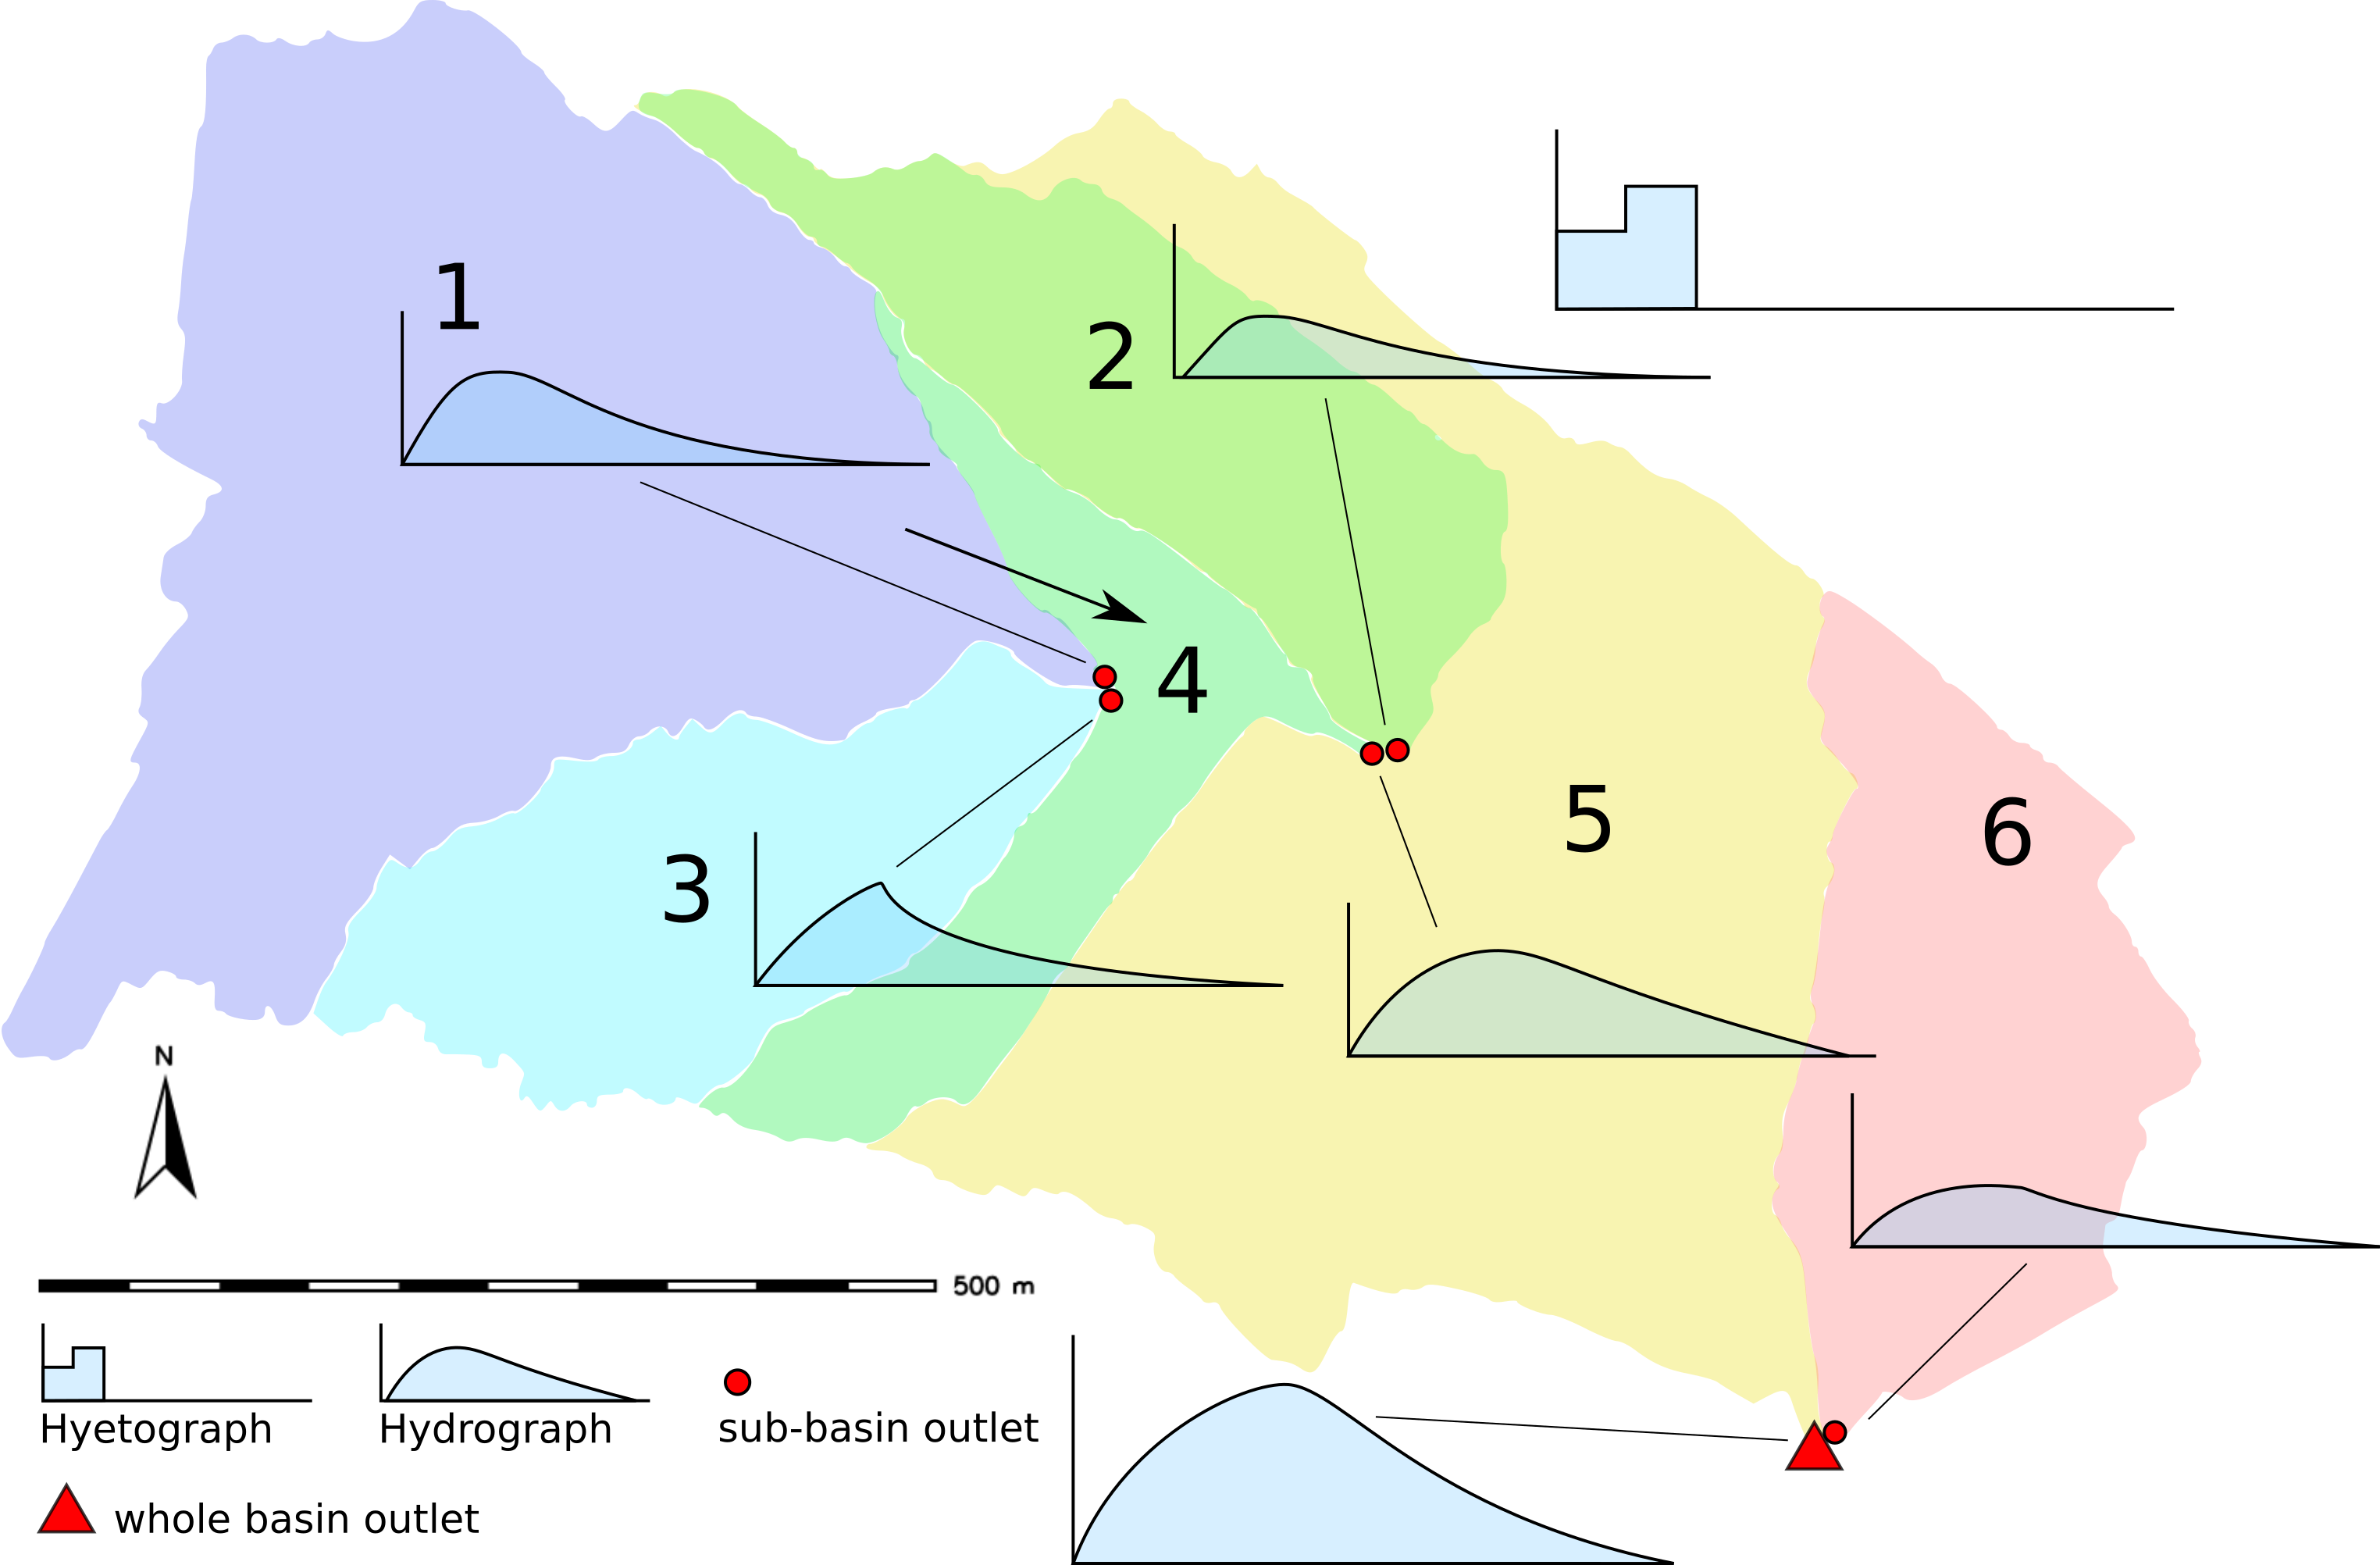
\includegraphics[width=0.9\columnwidth]{figures/smoderp-cpu-parallel.png}
    \caption{Simple example of possible CPU-based parallelization strategy for the experimental catchment Nu\v{c}ice}
    \label{fig:cpu-parallel}
  \end{center}
\end{figure}

The strategy main goal is the reduction of
the communication between CPU-cores during the computation as much as
possible. The whole basin is divided into several sub-basins based on
the digital elevation model and user-defined sub-basin size. 
Outlet\footnote{The location in the basin where all water from the basin flows} 
of each sub-basin is depicted with
red dots in Figure~\ref{fig:cpu-parallel}. After the sub-basins
are defined, an order in which each sub-basin will be computed is defined as
follows. Sub-basins which are hydrologically the farthest from the
basin outlet (depicted by the triangle in Figure~\ref{fig:cpu-parallel}) 
and therefore have no inflow flow upslope area are
calculated at first. Those sub-basins have the rainfall stored in
hyetographs as the only input. In the simplified setup shown in
Figure~\ref{fig:cpu-parallel}, the sub-basins 1, 2, 3, and 6 are
calculated at first in parallel. The calculated hydrographs of the
sub-basins 1, 2, 3, and 6 are stored in the memory for the later use. 
Sub-basins which have sub-basins 1, 2, 3, and 6 in its upslope area 
are calculated next. 
It this case it is the only the sub-basin 4. The water inputs in
the sub-basin 4 are now hyetograph and also hydrographs of
upslope sub-basins 1 and 3. 
Next sub-basin to be calculated is the final sub-basin 5. 
In this sub-basin is the outlet of the whole area.
The water input in the final sub-basin 5 are hyetograph and hydrographs 
of sub-basins 2, 4 and 6. Once the main outlet hydrograph is obtained 
the calculation stores the results and stops. 

This approach may encounter several limitations. The main one
originates from the basin geometry. In the case of a narrow basin
situation (each sub-basin has a single upslope and downslope
sub-basin), the sub-basins will be computed in a sequence, which loses
the advantage of multi-core working station. If this situation happens
the user will be forced to create very small sub-basins in order to be
able to perform the outlined CPU parallelization. The possibilities of
CPU parallelization described in this section will be the subject of
further research.
